\subsection{Gráfico}

Quando se deseja traçar o gráfico, ao menos um esboço, de uma função polinomial qualquer 
$p(x) = a_n x^n+ a_{n-1} x^{n-1} + \dots + a_1x + a_0$, certas informações são de grande utilidade. 
Algumas delas são:
%
\begin{itemize}
  \item Se $n$ é par, então para $\modu x $ suficientemente grande,
  $p(x)$ tem o mesmo sinal de $a_n$;
  \item Se $n$ é ímpar, então $p(x)$ tem o mesmo sinal de $a_n$ para
  valores positivos  muito grandes de $x$ e tem o sinal oposto de
  $a_n$ para valores negativos muito grandes, em módulo, de $x$.
\end{itemize}

\begin{example}
Identifique se $n$ é par ou ímpar e qual o sinal de $a_n$ para cada
um dos gráficos de funções polinomiais $p(x) = a_n x^n+ a_{n-1}
x^{n-1} + \dots + a_1x + a_0$ abaixo:

\begin{figure}[H]
  \centering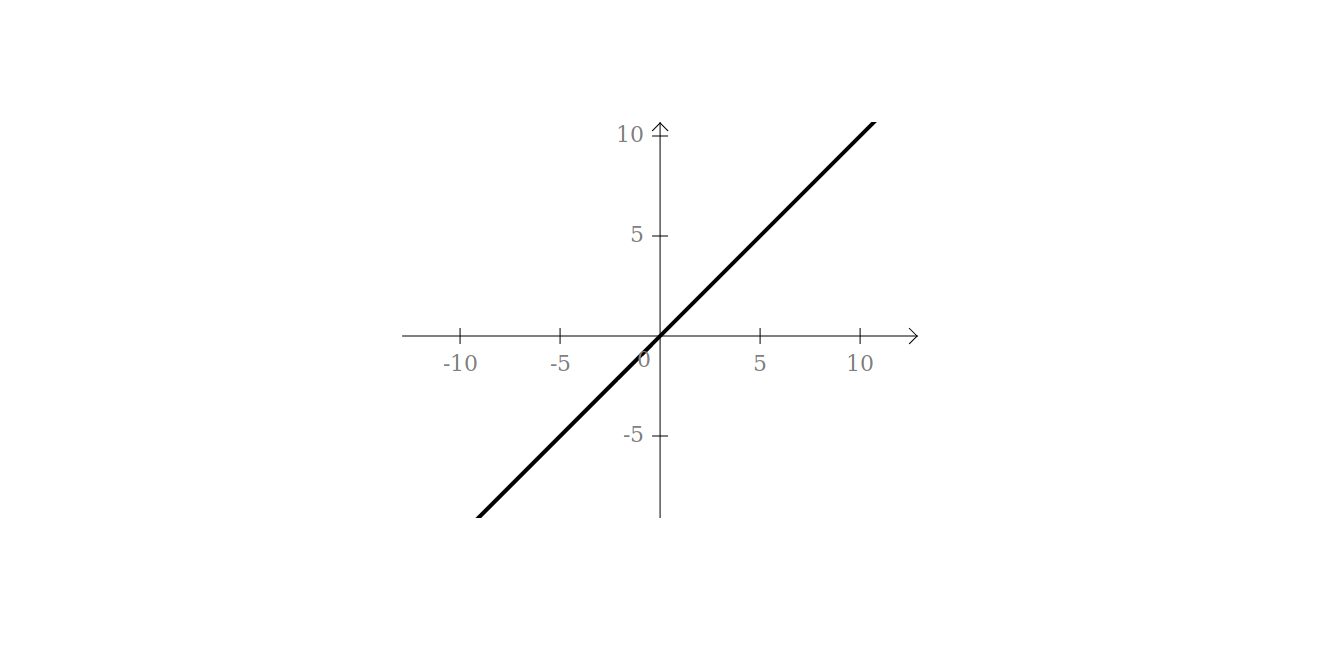
\includegraphics[scale=0.30]{\imgdirfromsection/polinomio-identidade.png}
\end{figure}

\begin{figure}[H]
  \centering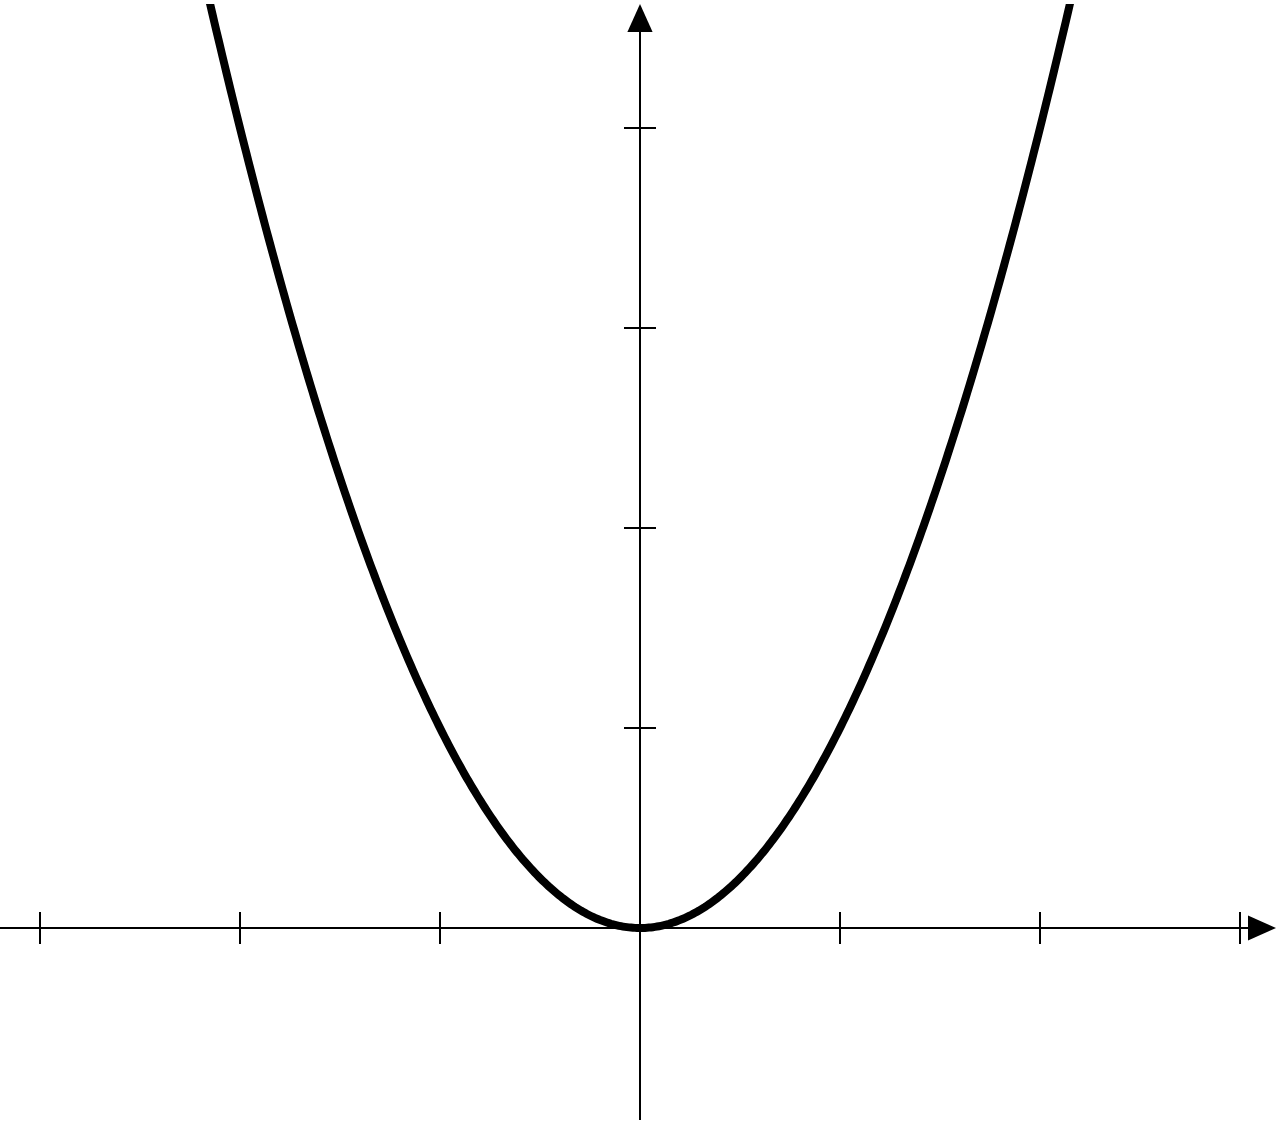
\includegraphics[scale=0.30]{\imgdirfromsection/polinomio-quadratico.png}
\end{figure}

\begin{figure}[H]
  \centering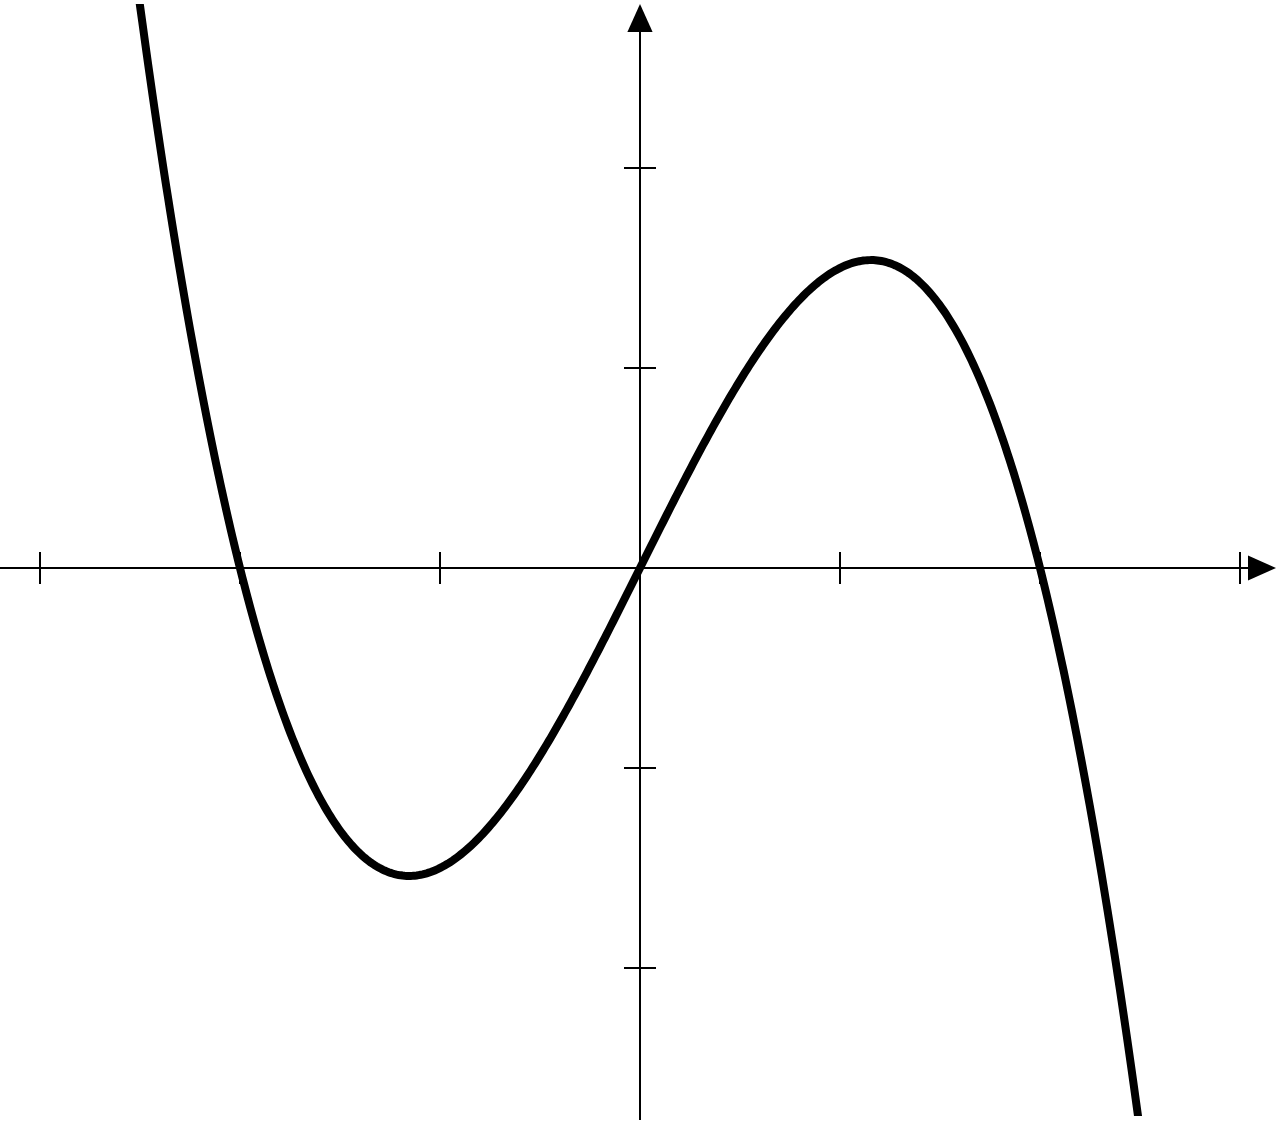
\includegraphics[scale=0.30]{\imgdirfromsection/polinomio-cubico.png}
\end{figure}

\begin{figure}[H]
  \centering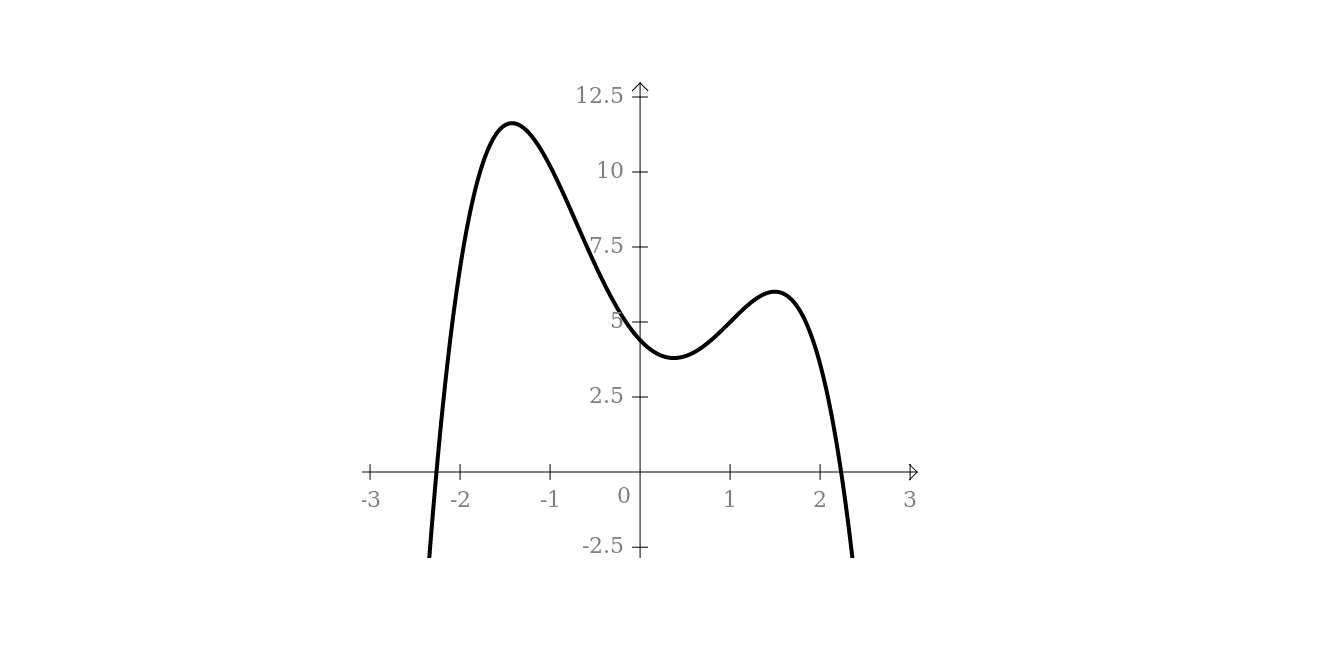
\includegraphics[scale=0.30]{\imgdirfromsection/polinomio-quarto-grau.png}
\end{figure}
\end{example}

Outros fatos que nos ajudam a traçar gráficos de funções polinomiais são:
%
\begin{itemize}
\item Se o grau de $p$ é maior do que o grau de outra função polinomial $q$, 
então para todo $x$ com valor absoluto suficientemente grande, 
tem-se $\modu {p(x)} > \modu{q(x)}$;
\item Sejam $x_1, x_2 \in \R$. Se $p(x_1) < 0$ e $p(x_2)>0$,
então, $p$ deve possuir uma raiz entre $x_1$ e $x_2$.
\end{itemize}

\begin{example}
Considere os polinômios $p(x) = x^7 $ e $q(x)=x^3$. 
Quando $0< \modu x < 1$, temos que $\modu {p(x)} < \modu{q(x)}$. 
Porém, quando $ \modu x > 1$, temos que $\modu {p(x)} > \modu{q(x)}$. 
Além disso, em ambos os casos, $p(-1) = q(-1) = -1 <0$ e $p(1) = q(1) = 1 >0$.
Assim, os polinômios possuem, cada um, ao menos uma raiz no
intervalo $(-1, 1)$ -- a saber, $x=0$.
\end{example}

\begin{onlineact}
    \khan{https://pt.khanacademy.org/math/algebra2/polynomial-functions/zeros-of-polynomials-and-their-graphs/e/using-zeros-to-graph-polynomials}
    {Zeros de Polinômios e seus Gráficos}.
\end{onlineact}